\documentclass[paper=a4, parskip=half]{scrreprt}

\usepackage{etex}
\usepackage[utf8]{inputenc}
\usepackage[T1]{fontenc}

\usepackage{lmodern}
\usepackage[ngerman]{babel}

\usepackage{bibgerm} 
\usepackage{cite}
\usepackage{url}

\usepackage{graphics}

\usepackage[hypertexnames=false, linktocpage]{hyperref}

\usepackage{titling}
\usepackage{graphicx}
\graphicspath{ {./Bilder/} }
\usepackage{wrapfig}
\usepackage{float}
\usepackage{adjustbox}
\usepackage{setspace}
\usepackage{hyperref}
\usepackage[acronym]{glossaries}
\usepackage{datetime}
\usepackage[normalem]{ulem}

\usepackage{subfiles} % Best loaded last in the preamble

\subfile{Meta/glossary}

\setcounter{tocdepth}{1}

\begin{document}
%TC:ignore
\title{Vision and Scope} % Meta

\subfile{Meta/coversheet}
\subfile{Meta/guides}


%Dieses Projekt ist Teil einer Studienarbeit der Hochschule für Wirtschaft und Recht Berlin. Das Projekt erzielt damit keine kommerzielle Absicht und dient als Lehrmethode für das Modul ''Software Engineering I''.
%Zu Beginn des Projekts gab es von den Betreuer*innen der Hochschule die Anforderung eines der 17 Sustainable Development Goals der United Nations \cite{UNGoals} zu erfüllen. Ebenso wurden Anforderungen zu Dokumentationsthemen und zeitliche Fristen gesetzt.


%TC:endignore
%Alternativ zu Geschäftlich würde auch Unternehmehrisch passen
\chapter{Geschäftliche Anforderungen}
\section{Hintergrund}
Das Gendern findet immer mehr Anwendung, insbesondere im pädagogischen, wie auch im akademischen Bereich. So werden unter anderem wissenschaftliche Arbeiten von Student*innen in genderneutraler Sprache verfasst, Artikel und Recherchen durch Journalist*innen werden genderneutral publiziert. Das Schreiben von genderneutralen Texten wirkt für viele zu Beginn recht schwer. Es gibt viele neue Begrifflichkeiten und Möglichkeiten, wie gegendert werden kann. Es bedarf einer individuellen Eingewöhnungszeit.


\section{Geschäftliche Möglichkeiten}
Unterschiedlichste Berufs- und Bildungsgruppen möchen inhaltlich saubere Arbeiten liefern und gleichzeitig einwandfrei und konsistent z.B. entweder mit Stern oder Doppelpunkt gendern. \textsc{Genderly} soll dahingehend viele Hürden nehmen. \textsc{Genderly} soll ein System werden, in das Nutzer*innen Text eingeben können. Zum Text erstellt es einen genderneutralen Vorschlag. Verfasser*innen behalten ihren Fokus so weiterhin auf inhaltlicher Arbeit, die Aufgabe des Genderns wird abgenommen.

\section{Geschäftliche Zielsetzungen}

\begin{table}[!htb]
\begin{tabular}{ll}
\textbf{Ziel 1} & Senkung des notwendigen Zeitaufwands für Texteditierung \\
 & um 25\% bis 50\%, bereits nach erstmaliger Nutzung. Aufwandssenkungen \\
 & sind dabei abhängig vom Textvolumen. \vspace{0.15cm} \\
\textbf{Ziel 2} & Senkung der mit der bisherigen Texteditierung verbundenen \\
 & Ressourcenbedarfe und Kosten, bereits nach erstmaliger Nutzung. \\
 & Senkungen wirken direkt proportional zur Dauer des Anwendungseinsatzes. \vspace{0.15cm} \\
\textbf{Ziel 3} & Realisierung eines Bildungs- und Lerneffektes durch generierte Text-\\
& vorschläge. Nach 10 einzelnen Nutzungen sollen Nutzer*innen einen\\
& sichereren Umgang mit Gendern zeigen. Texte können durch sie mit\\
& einer 50\% geringeren Fehlerwahrscheinlichkeit selbstständig gegendert werden.\\

%\textbf{Ziel 1} & Weboberfläche schaffen mit einer Textbox für den Eingabetext und einer \\
% & Textbox für den Ausgabetext und einen Bestätigungknopf \vspace{0.15cm} \\
%\textbf{Ziel 2} & Erstellen und Einbinden eines Datenbankmodells \vspace{0.15cm} \\
%\textbf{Ziel 3} & Füllen der Datenbank mit Datensätzen \vspace{0.15cm} \\
%\textbf{Ziel 4} & Anbindung an die Datenbank \vspace{0.15cm} \\
%\textbf{Ziel 5} & Algorithmische Analyse des Eigabetexts inklusive Ausgabe eines\\
% & genderneutralen Vorschlags \\
\end{tabular}
\end{table}


\section{Erfolgsmetriken}
% X Amount of green unit tests?
% Beispielsätze bei denen eine Genderneutralervorschlag erwartet wird
\begin{table}[!htb]
\begin{tabular}{ll}
\textbf{Metrik 1} & Drei Monate nach Release steigt die Anzahl wiederkehrender Nutzer*innen\\
& auf ein Sechsfaches des ersten Monats. Das impliziert, dass Bedürfnisse der\\ % Sechsfaches wirklich groß
& Zielgruppe erfüllt werden und wiederkehrende Nutzer*innen zufrieden sind.\\
& Zudem weist der Faktor indirekt darauf hin, dass Nutzer*innen wahrschein-\\
& lich bereit sind, die App weiterzuempfehlen. \vspace{0.15cm} \\ % wird wirklich so geschrieben
\textbf{Metrik 2} & Sechs Monate nach Release steigt die Anzahl erstmaliger Nutzer*innen auf\\
& ein Vierfaches des dritten Monats. Das impliziert, dass Nutzer*innen der\\
& Zielgruppen bedarfsgerecht angesprochen werden und, dass durch \textsc{Genderly} \\
& tatsächlicher Mehrwert geschaffen wird.\vspace{0.15cm} \\
\end{tabular}
\end{table}

\section{Vision Statement} % needs better translation

\textsc{Genderly} ist eine Web-App, zur Texterfassung, -analyse und Generierung eines genderneutralen Vorschlagstexts, basierend auf einem eingegebenen Text. Sie widmet sich der Geschlechtergleichheit in unser aller Sprache. Die App kann möglichst einfach über eine Vielzahl unterschiedlicher Endgeräte erreicht und genutzt werden. Die Zielgruppe besteht aus all denjenigen Menschen, die in ihrer Arbeit Bedarf für Automatisierung und Erlernen des Genderns von Texten sehen. Aufgrund besonders hohen Bedarfs ist die App allerdings vorrangig an Anforderungen des akademischen, des pädagogischen und des journalistischen Raums angepasst.\\
Die App nimmt syntaktisch korrekten Text auf, verarbeitet ihn mithilfe von Referenzeinträgen in einer Datenbank und findet und ersetzt ggf. Substantive und mit ihnen assoziierte Artikel. Die breite Fächerung und Diversität der Einsatzbereiche, in denen \textsc{Genderly} so einen Mehrwert leisten kann, erfordert eine besonders übersichtliche, einfache Aufmachung und Steuerbarkeit der App. Nutzer*innen können Texte eingeben, Sprache (z.B. Deutsch, Englisch, etc.), sowie Gendering-Stil (z.B. Doppelpunkt-, Sternchen-Schreibweise, gänzlicher Wortersatz, etc.) einstellen und erhalten den Vorschlagstext gegenüber dem Eingabetext dargestellt.\\
Funktionsweise, Aufmachung und Gegenüberstellung machen \textsc{Genderly} nicht nur zu einer Arbeitshilfe, sondern auch zu einem Lernmittel für korrektes Gendern.

\pagebreak

\section{Geschäftliche Risiken}

\begin{table}[!htb]
\begin{tabular}{ll}
\textbf{Risikofaktor 1} & Gendering-Stile können sich ändern, Nutzer*innen könnten nicht\\
& unterstützten Gendering-Stil verlangen. Sie müssten im Zweifel \\
& improvisieren oder größere Änderungen an Vorschlagstexten vornehmen. \vspace{0.15cm} \\
& \textit{(Wahrscheinlichkeit = 0,4; Auswirkung = 6)} \vspace{0.15cm} \\
\textbf{Risikofaktor 2} & Zu wenige Nutzer*innen verwenden die App. Das verkleinert den\\
 & Return on Investment des Projekts. Durch \textsc{Genderly} angesprochene\\
 & Arbeitsabläufe blieben unverändert und damit teurer.\vspace{0.15cm} \\
 & \textit{(Wahrscheinlichkeit = 0,3; Auswirkung = 9)} \vspace{0.15cm} \\
\textbf{Risikofaktor 3} & Durch Nutzer*innen verwendete Sprachen sind nicht unterstützt. Die\\
 & App wird nicht unbenutzbar, Nutzer*in könnte über Umwege und durch \\
 & Drittanbieter-Lösungen die unterstützten Sprachen zur Zielsprache \\
 & übersetzen lassen. \vspace{0.15cm} \\
 & \textit{(Wahrscheinlichkeit = 0,4; Auswirkung = 7)} \vspace{0.15cm} \\
\end{tabular}
\end{table}

\section{Geschäftliche Annahmen und Abhängigkeiten}

\begin{table}[!htb]
\begin{tabular}{ll}
\textbf{Annahme 1} & Benutzer*innen geben mindestens einen Satz ein. \vspace{0.15cm} \\
\textbf{Annahme 2} & Benutzer*innen geben Text syntaktisch korrekt ein. \vspace{0.15cm}\\
\textbf{Annahme 3} & Nutzer*innen haben Zugang zu einem internetfähigen Gerät. \vspace{0.15cm} \\
\textbf{Annahme 4} & Die Web-App wird auf einem dem Anfragevolumen gerecht \\
& werdenden System betrieben. \vspace{0.15cm} \\
\end{tabular}
\end{table}

\begin{table}[!htb]
\begin{tabular}{ll}
\textbf{Abhängigkeit 1} & Benutzer*innen verfügen über einen Internetzugang. \vspace{0.15cm} \\
\textbf{Abhängigkeit 2} & Wenn Benutzer*innen internetfähige Geräte, wie z.B. \\
& Smartboards oder Tablets nutzen, muss \textsc{Genderly}\\
& mit diesen Geräten kompatibel sein. \vspace{0.15cm}\\
\end{tabular}
\end{table}

\chapter{Geltungsbereich und Grenzen}
\section{Grundfunktionalitäten}
\label{sec:Grundfunktionalitäten}

\begin{table}[!htb]
\begin{tabular}{ll}
\textbf{Funktionalität 1} & Aufrufbarkeit der Anwendung über eine eigene Weboberfläche. \vspace{0.1cm} \\
\textbf{Funktionalität 2} & Aufnahme von Text über eigenes Eingabefeld. \vspace{0.1cm} \\
\textbf{Funktionalität 3} & Auswahlmöglichkeiten für die Sprache des Texts. \vspace{0.1cm} \\
\textbf{Funktionalität 4} & Auswahlmöglichkeiten für den Gendering-Stil des durch eine \\
 & Analyse auszugebenden Text-Vorschlags. \vspace{0.1cm} \\
\textbf{Funktionalität 5} & Ermittlung und ggf. Austausch genderbarer Substantive. \vspace{0.1cm} \\
\textbf{Funktionalität 6} & Ermittlung und ggf. Austausch durch Gendering \\
& verfälschter Artikelzuordnungen. \vspace{0.1cm} \\
\textbf{Funktionalität 7} & Anpassung der farblichen Darstellung durch Nutzer*innen \vspace{0.1cm} \\
\textbf{Funktionalität 8} & Visualisierung des Ausgabetextes, sodass Nutzer*innen den \\
 & Ausgabetext noch nachbearbeiten können. \vspace{0.1cm} \\
\end{tabular}
\end{table}

\begin{figure}[hbt!]
  \centering
  \fbox{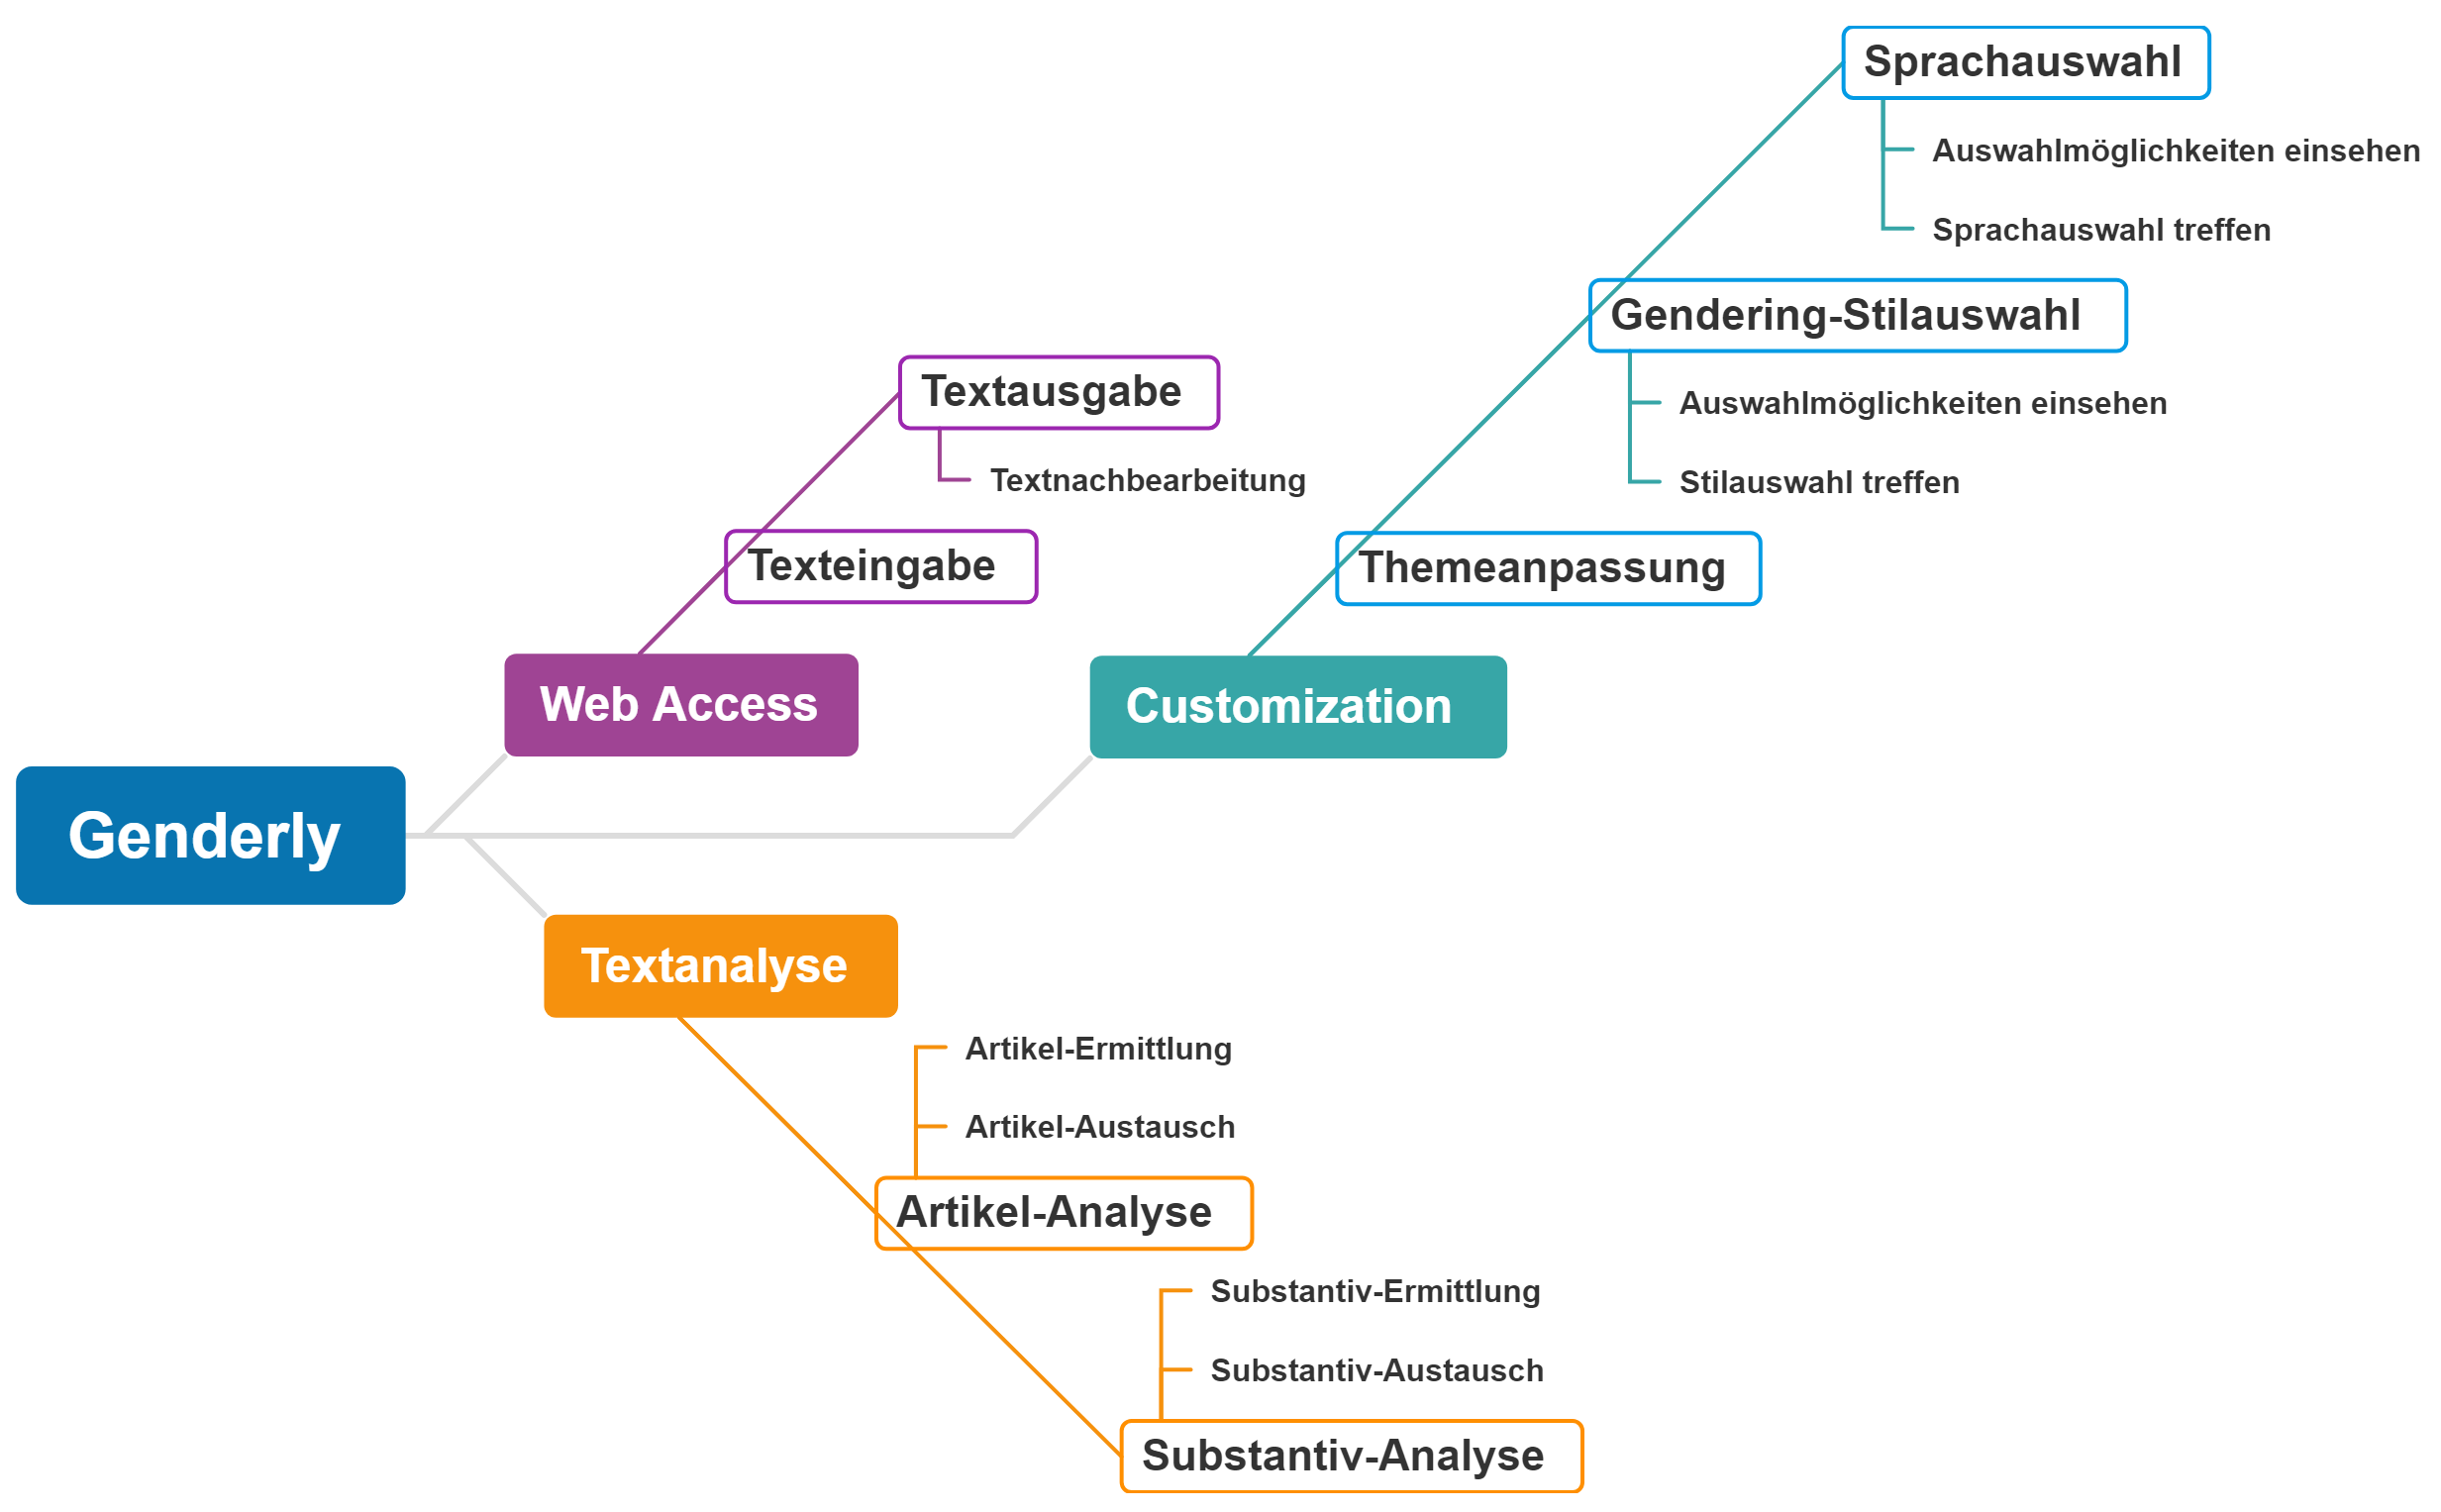
\includegraphics[scale=0.205]{Bilder/Genderly_FeatureTree.png}}
  \vspace{-0.25cm}
  \caption[Partieller Feature Tree]{Partieller Feature Tree}
  \label{fig:Bahn-RBC}
\end{figure}

%Die Grundfunktionalität besteht aus einer Weboberfläche mit Zwei Textboxen und einen Knopf zur Bestätigung der Eingabe.
%Eine Textbox lässt die Eingabe zu in welcher der zu verarbeitende Text enthalten ist. Die Zweite Textbox liefert nach der Bestätigung der Eingabe einen Textlichen Vorschlag einer genderneutralen Variante des zuvor eingegebenen Textes.

\section{Umfang der ersten Lieferung}

Die erste Lieferung besteht nicht aus einer vollständig realisierten und zu veröffentlichenden Anwendung. Sie stellt einen Prototyp für eine Teilmenge der unter \ref{sec:Grundfunktionalitäten}: \nameref{sec:Grundfunktionalitäten} aufgestellten Features dar. Im Folgenden ist die Auflistung dieser Funktionalitäten zu finden.

\begin{table}[!htb]
\begin{tabular}{ll}
\textbf{Funktionalität 1} & Aufrufbarkeit der Anwendung über eine eigene Weboberfläche. \vspace{0.1cm} \\
\textbf{Funktionalität 2} & Aufnahme von Text über eigenes Eingabefeld. \vspace{0.1cm} \\
\sout{\textbf{Funktionalität 3}} & \sout{Auswahlmöglichkeiten für die Sprache des Texts.} \vspace{0.1cm} \\
\sout{\textbf{Funktionalität 4}} & \sout{Auswahlmöglichkeiten für den Gendering-Stil des durch eine} \\
 & \sout{Analyse auszugebenden Text-Vorschlags.} \vspace{0.1cm} \\
\textbf{Funktionalität 5} & Ermittlung und ggf. Austausch genderbarer Substantive. \vspace{0.1cm} \\
\textbf{Funktionalität 6} & Ermittlung und ggf. Austausch durch Gendering \\
& verfälschter Artikelzuordnungen. \vspace{0.1cm} \\
\sout{\textbf{Funktionalität 7}} & \sout{Anpassung der farblichen Darstellung durch Nutzer*innen} \vspace{0.1cm} \\
\textbf{Funktionalität 8} & Visualisierung des Ausgabetextes, sodass Nutzer*innen den \\
 & Ausgabetext noch nachbearbeiten können. \vspace{0.1cm} \\
\end{tabular}
\end{table}

\section{Umfang der nachträglichen Lieferungen}

Nachträgliche Lieferungen sollen in erster Linie zur Komplettierung der verfügbaren Grundfunktionlitäten dienen. Darüber hinaus bieten sich für \textsc{Genderly} beispielsweise Möglichkeiten der Monetarisierung durch Werbung an. Zukünftige Lieferungen können in noch nicht festgelegter Reihenfolge die hier aufgeführten Funktionalitäten beitragen:

\begin{table}[!htb]
\begin{tabular}{ll}
\textbf{Nachtrag 1} & Auswahlmöglichkeiten für die Sprache des Texts. \vspace{0.1cm} \\
\textbf{Nachtrag 2} & Auswahlmöglichkeiten für den Gendering-Stil des durch eine \\
 & Analyse auszugebenden Text-Vorschlags. \vspace{0.1cm} \\
\textbf{Nachtrag 3} & Anpassung der farblichen Darstellung durch Nutzer*innen \vspace{0.1cm} \\
\textbf{Nachtrag 4} & Premium-Modus, wobei die kostenlose Nutzung auf \\
& eine maximale Wortmenge begrenzt wird. \vspace{0.1cm} \\
\textbf{Nachtrag 5} & Darstellung von Werbeinhalten zwecks Monetarisierung. \vspace{0.1cm} \\
\end{tabular}
\end{table}

In Absprache mit den Stakeholder*innen werden diese möglichen Freatures je Release-Zyklus priorisiert implementiert oder gar verworfen.

\section{Begrenzungen und Abgrenzungen}
Gendern findet über die deutsche Sprache hinaus auch in anderen Sprachen Verwendung. Aufgrund der Einschränkungen in Umfang, Zeit und Teamgröße wird auf das Implementieren von Analyse-Logik für mehrere Sprachen vorerst verzichtet. Der Prototyp soll allein deutschen Text verarbeiten.\\
Die Anwendung hat nicht das Ziel, in jeder Situation einen syntaktisch und grammatikalisch korrekten Satz zu bilden, welcher inhaltlich nicht vom originalen Text abweicht. Bei dem erzeugten Text handelt es sich allein um einen Vorschlag. Dieser dient nur als Assistenz, als Hilfestellung und Möglichkeit zur Weiterbildung.\\
Ebenso hat die Anwendung nicht das Ziel, mit grammatikalischen oder rechtschreiblichen Fehlern im Eingabetext einen genderneutralen, grammatikalisch absolut korrekten Satz syntaktisch korrekt und ohne Rechtschreibfehler im Ausgabetext als Vorschlag zu bilden. Der Ausgabetext soll auch hinsichtlich dieser Eigenschaft prototypischen Vorschlagscharakter besitzen.

\chapter{Geschäftskontext}
\section{Profile von Interessengruppen}

Alle Interessensgruppen wurden sehr ausführlich in der bestehenden Stakeholder-Analyse zusammengefasst.
Im Nachfolgenden befindet sich daher nur noch eine sehr grobe Zusammenfassung.

\begin{tabular}
	{
		|p{0.2\textwidth}
		|p{0.2\textwidth}
		|p{0.2\textwidth}
		|p{0.2\textwidth}
		|p{0.25\textwidth}
		|
	}
	\hline
		\textbf{Stakeholder}
	&\textbf{Ziele}
	&	\textbf{Einstellung}
	&	\textbf{Interessen}
	&	\textbf{Einschränkungen}\\
	\hline
	Entwickler*innen
	&Zukunftssicheres lauffähiges Produkt welche alle Anforderungen erfüllt
	&Hohes Interesse an pünktlicher, vollumfänglicher Ergebnislieferung
	&Fehlerquote der Textvorschläge muss möglichst gering sein
	&Begrenztes Zeitbudget für Entwicklung\\
	\hline
	
	Gesetzgeber*innen
&Die Gesetzgeber*innen haben kein direktes Interesse am Produkt. Für sie ist wichtig,
dass gegen keine Gesetze verstoßen wird.
&Keine hohe Affinität für Web-Technologien, dennoch Motivation durch dringenden Bedarf der Funktionalität
&Problemloses Regieren und Regulieren
&Verstöße müssen angezeigt und ihre Auswirkungen korrigiert werden.\\
\hline

	Anwender*innen des Systems
&Lauffähiges Produkt
&In Anwendung wird dringend notwendiger Beitrag für Geschlechtergleichberechtigung im Alltag gesehen
&Leichtes Erlernen und Anwenden der Software
&Keine Gefunden\\
\hline

	Product-Owner
&Erfolgreiches Abschließen des Projekts
&Starkes Interesse für pünktliche Bereitstellung gegenüber einer größtmöglichen Menge an Nutzer*innen
&Die Erfüllung eines der 17 Sustainable Development Goals der United Nations \cite{UNGoals}
&Keine Gefunden\\
\hline


\end{tabular}


\section{Prioritäten des Projekts}

	\begin{tabular}
	{
		|p{0.2\textwidth}
		|p{0.2\textwidth}
		|p{0.2\textwidth}
		|p{0.4\textwidth}
		|}
	\hline
	\textbf{}
	&\textbf{Hauptziele}
	&\textbf{Bedingungen}
	&\textbf{Freiheiten}\\
	\hline
	\textbf{Funktionalität}
	&Erfüllung aller Anforderungen für die erste Lieferung
	&4 Entwickler
	&Nach Absprache in der Gruppe\\
	\hline
		\textbf{Qualität}
	&Textvorschlag beinhaltet genderneutrale Form (Grammatik kann abweichen)
	&4 Tester + Automatisierte Tests decken den Analyse-Prozess und die Logik zur Web-Oberfläche ab
	&Anforderungen müssen Mindestmaß erfüllen\\
	\hline
		\textbf{Zeitraum}
	&27.08.2021 - 04.11.2021 wird eingehalten
	& Mitarbeit aller 4 Teammitglieder
	&Keine\\
	\hline
		\textbf{Kosten}
	&0€ - Free
	&Hardware für Prototyp-Betrieb kostenfrei nutzbar
	&Nach Absprache in der Gruppe kann zum Beispiel eine Domain erworben werden\\
	\hline
		\textbf{Mitarbeiter}
	&Lernwert für alle 4 Teammitglieder
	&Mitarbeit aller 4 Teammitglieder
	&Keine\\
	\hline


\end{tabular}


\section{Anwendungsbereitstellung}
Die Anwendung zielt besonders auf die Verwendung im akademischen, wissenschaftlichen und pädagogischen Kontext ab. Sie wird daher voraussichtlich über einen Webbrowser primär auf mobilen Endgeräten Einsatz finden. Weitere mögliche Geräte sind Smartboards und auch stationäre Rechner, beispielsweise in universitären Laborräumen.\\
Das Frontend muss dahingehend hohe Kompatibilität aufweisen und flexibel für diese unterschiedlichen Endgeräte erreichbar sein. Die genutzten Web-Standards müssen aktuell sein. Es bedarf auch eines wohl dimensionierten Backends, das die gewünschten Funktionalitäten mit möglichst hoher Geschwindigkeit für die Nutzer abwickelt. Nutzerseitig soll kein Training für die Bedienung der Anwendung notwendig sein, da die App intuitiv aufgebaut ist.
%TC:ignore

%Glossar
\printglossary
\pagebreak

\nocite{*}
\bibliography{Literatur}
\bibliographystyle{alphadin}


\subfile{Anhang/main}
%TC:endignore

\end{document}